\documentclass[11pt]{article}

\usepackage{amsmath}
\usepackage{amssymb}
\usepackage[margin = 2.5cm]{geometry}
\usepackage{graphicx}

\usepackage{sectsty}
\sectionfont{\fontsize{12}{16}\selectfont\centering}
\subsectionfont{\fontsize{10}{14}\selectfont}

\usepackage{natbib}
\bibliographystyle{apalike}

\usepackage{hyperref}
\hypersetup{colorlinks,linkcolor={blue},citecolor={blue},urlcolor={blue}}  


\author{Gregor Steiner}
\title{Master Thesis Proposal}

\begin{document}

\maketitle

\section*{Idea}

I would like to estimate the causal effect of heatwaves on labor productivity. My idea is exploiting the 2021 heatwave on the North American west coast (see figure 1). 

\begin{figure}[h]
	\centering
	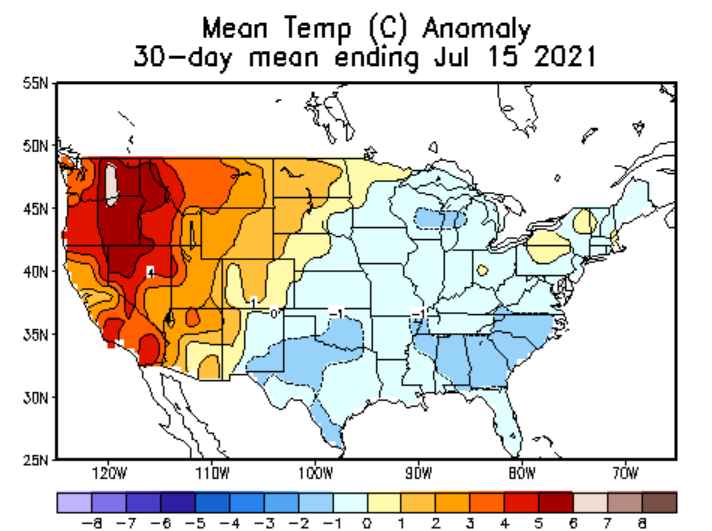
\includegraphics[scale = 0.6]{TempAnomMap}
	\caption{Mean temperature anomalies in June/July 2021 (Source: \href{https://www.cpc.ncep.noaa.gov/products/tanal/temp_analyses.php}{National Weather Service})}
\end{figure}


\section*{Empirical Strategy}

I would like to use a synthetic control approach based on \citet{Abadie2003} and \citet{Abadie2021}. The treated states would be Idaho, Oregon and Washington (maybe also California and Nevada?). For each of those I would create a synthetic control group where the donor pool consists of the other 47 (or 45?) states. If data availability allows, I could incorporate Canadian provinces as well, since British Columbia was also hit hard by the heatwave.

The outcome would be some measure of labor productivity. Unfortunately a traditional output relative to hours worked measure is usually only available quarterly. The effect (if it is there) should be visible in quarter 2 and 3 of 2021 (see figure 2). But since the heatwave was only active for about 2 weeks, this will probably not work.

That's why I want to use  an unconventional proxy for labor productivity, which is available at a higher frequency. One idea would be Google searches for typical procrastination activities or social media activity during work hours. Of course, such measures would only be applicable to office jobs, where work is predominantly done on a computer (service industry?). 


\begin{figure}[h]
	\centering
	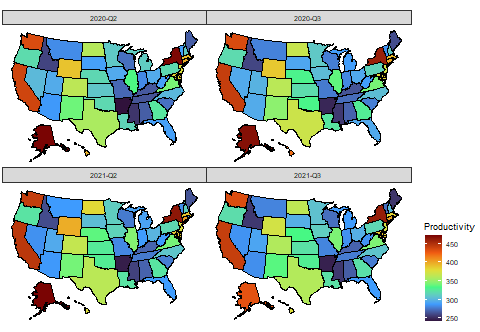
\includegraphics[scale = 0.8]{ProdMap}
	\caption{Output per hour worked by state (Source: BLS, FRED and own calculations)}
\end{figure}





\bibliography{references}

\end{document}
